\documentclass[a4paper,12pt]{article}

% Paquetes necesarios
\usepackage[utf8]{inputenc} % Codificación UTF-8
\usepackage[spanish]{babel} % Idioma español
\usepackage{amsmath, amssymb} % Matemáticas
\usepackage{graphicx} % Imágenes
\usepackage{geometry} % Configuración de márgenes
\usepackage{fancyhdr} % Encabezados y pies de página
\usepackage{titlesec} % Formato de títulos
\usepackage{enumitem} % Listas personalizadas

% Configuración de márgenes
\geometry{top=2.5cm, bottom=2.5cm, left=3cm, right=3cm}

% Configuración de encabezados y pies de página
\pagestyle{fancy}
\fancyhf{}
\fancyhead[L]{\textit{Proyecto de Simulación}}
\fancyhead[R]{\thepage}
\fancyfoot[L]{Autor: Eveliz Espinaco Milián}
\fancyfoot[R]{\today}

% Configuración de títulos
\titleformat{\section}{\large\bfseries}{\thesection.}{1em}{}
\titleformat{\subsection}{\normalsize\bfseries}{\thesubsection.}{1em}{}

% Información de la portada
\title{
    \vspace{2cm}
    \textbf{\Huge Proyecto de Simulación de Eventos Discretos} \\
    \vspace{1cm}
    \large Tema:  Modelo de inventario \\
    \vspace{2cm}
}
\author{[Tu Nombre] \\ [Tu Institución] \\ [Tu Correo Electrónico]}
\date{\today}

\begin{document}
% Portada
\begin{titlepage}
    \centering

    % Título principal
    {\huge\bfseries Proyecto de Simulación de eventos discretos \par}
    \vspace{0.5cm}
    {\Large Tema:  Modelo de inventario \par}
    \vspace{1.5cm}

    % Logo principal

    % Información del autor
    \vspace{1cm}
    \textbf{Autor:} Eveliz Espinaco Milián \par
    \textbf{Carrera:} Ciencia de la Computación, tercer año\par
    \vfill

    % Logo secundario y universidad
    
\includegraphics[width=0.2\textwidth]{./img/MATCOM.jpg} \\[0.5cm]
    {\scshape\Large Facultad de Matemática y Computación \par}
    {\scshape\large Universidad de La Habana, Cuba \par}

    % Fecha
    \text \today \par
\end{titlepage}

\section{Introducción}
El proyecto consiste en la simulación de un sistema de gestión de inventarios bajo la política \textbf{(s, S)}, donde una tienda reabastece su inventario cuando este cae por debajo de un nivel mínimo \( s \), solicitando una cantidad suficiente para alcanzar un nivel máximo \( S \). El objetivo principal es evaluar la rentabilidad del sistema considerando ingresos por ventas, costos de pedidos y costos de mantenimiento de inventario. La simulación utiliza un enfoque de \textbf{eventos discretos} para modelar la dinámica del sistema, incluyendo la llegada aleatoria de clientes, la demanda variable y los tiempos de entrega de los pedidos.

\subsection*{Objetivos y Metas}
\begin{itemize}
    \item \textbf{Objetivo General}:  
    Estimar la \textbf{ganancia esperada por unidad de tiempo} bajo diferentes políticas de inventario \((s, S)\).
    \item \textbf{Metas Específicas}:
    \begin{itemize}
        \item Analizar el impacto de los niveles \( s \) y \( S \) en los costos operativos y la rentabilidad.
        \item Evaluar la sensibilidad del sistema ante cambios en parámetros clave (ej: tasa de llegada de clientes, tiempo de entrega).
        \item Identificar la política óptima \((s, S)\) que maximice la ganancia neta.
    \end{itemize}
\end{itemize}

\subsection*{Sistema a Simular}
Se modela un sistema de inventario con las siguientes características:
\begin{itemize}
    \item \textbf{Eventos discretos}:
    \begin{itemize}
        \item \textbf{Llegada de clientes}: Ocurren según un proceso de Poisson con tasa \( \lambda \). Cada cliente demanda una cantidad aleatoria con distribución \( G \).
        \item \textbf{Llegada de pedidos}: Tardan \( L \) unidades de tiempo en ser entregados.
    \end{itemize}
    \item \textbf{Mecánica de reorden}:
    \begin{itemize}
        \item Si el inventario \( x < s \) y no hay pedidos pendientes (\( y = 0 \)), se solicita \( S - x \) unidades.
    \end{itemize}
    \item \textbf{Costos asociados}:
    \begin{itemize}
        \item Costo de pedido \( c(y) \).
        \item Costo de mantenimiento \( h \) por unidad de inventario por unidad de tiempo.
        \item Ingresos por venta a precio unitario \( r \).
    \end{itemize}
\end{itemize}

\subsection*{Variables del Problema}
\begin{itemize}
    \item \textbf{Parámetros del modelo}:
    \begin{itemize}
        \item \( r \): Precio de venta unitario.
        \item \( \lambda \): Tasa de llegada de clientes (proceso Poisson).
        \item \( G \): Distribución de la demanda por cliente.
        \item \( s \): Nivel mínimo de reorden.
        \item \( S \): Nivel objetivo de inventario.
        \item \( c(y) \): Función de costo por pedido de \( y \) unidades.
        \item \( L \): Tiempo de entrega de pedidos.
        \item \( h \): Costo de mantenimiento por unidad de inventario por unidad de tiempo.
        \item \( T \): Tiempo total de simulación.
    \end{itemize}
    \item \textbf{Variables de estado}:
    \begin{itemize}
        \item \( x \): Inventario actual disponible.
        \item \( y \): Cantidad de unidades pedidas y pendientes de entrega.
    \end{itemize}
    \item \textbf{Variables de conteo}:
    \begin{itemize}
        \item \( C \): Costo acumulado de pedidos.
        \item \( H \): Costo acumulado de mantenimiento.
        \item \( R \): Ingresos acumulados por ventas.
    \end{itemize}
    \item \textbf{Métrica clave}:
    \begin{itemize}
        \item Ganancia promedio por unidad de tiempo: \( \frac{R - C - H}{T} \).
    \end{itemize}
\subsection*{Variables de Interés para Análisis}
Cada equipo deberá analizar, entre otras:
\begin{itemize}
    \item Niveles óptimos \( s \) y \( S \).
    \item Sensibilidad del sistema al tiempo de entrega \( L \).
    \item Impacto de la variabilidad en la demanda (\( G \)) en la rentabilidad.
    \item Efecto de la tasa de llegada de clientes (\( \lambda \)) en los costos operativos.
\end{itemize}

\subsection*{Pasos seguidos para la implementación}
\begin{enumerate}
    \item \textbf{Inicialización de Parámetros}:
    \begin{itemize}
        \item Se definieron los parámetros del modelo:
        \begin{itemize}
            \item \( r \), \( \lambda \), \( s \), \( S \), \( L \), \( h \), \( T \).
            \item Funciones: \( G \) (generador de demanda) y \( c \) (función de costo de pedido).
        \end{itemize}
        \item Se inicializaron las variables de estado (\( x \), \( y \)) y las variables de conteo (\( C \), \( H \), \( R \)).
    \end{itemize}

    \item \textbf{Manejo de Eventos Discretos}:
    \begin{itemize}
        \item \textbf{Eventos principales}:
        \begin{itemize}
            \item \textbf{Llegada de clientes}: Generados mediante un proceso Poisson con tiempo entre llegadas exponencial (\( t_0 \)).
            \item \textbf{Entrega de pedidos}: Programados en \( t_1 = t + L \) al realizar un pedido.
        \end{itemize}
        \item \textbf{Lógica de procesamiento}:
        \begin{itemize}
            \item En cada iteración, se compara \( t_0 \) (próximo cliente) y \( t_1 \) (próximo pedido) para determinar cuál evento ocurre primero.
        \end{itemize}
    \end{itemize}

    \item \textbf{Procesamiento de Casos}:
    \begin{itemize}
        \item \textbf{Caso 1: Llegada de cliente (\( t_0 < t_1 \))}
        \begin{enumerate}
            \item Actualizar costos de mantenimiento acumulados.
            \item Generar demanda aleatoria \( D \).
            \item Calcular venta efectiva (\( w = \min(D, x) \)).
            \item Actualizar inventario (\( x = x - w \)) e ingresos (\( R += w \cdot r \)).
            \item Si \( x < s \) y no hay pedido pendiente (\( y = 0 \)):
            \begin{itemize}
                \item Realizar pedido (\( y = S - x \)).
                \item Programar entrega (\( t_1 = t + L \)).
            \end{itemize}
            \item Generar próximo tiempo de llegada de cliente (\( t_0 \)).
        \end{enumerate}

        \item \textbf{Caso 2: Entrega de pedido (\( t_1 \leq t_0 \))}
        \begin{enumerate}
            \item Actualizar costos de mantenimiento acumulados.
            \item Añadir unidades pedidas al inventario (\( x += y \)).
            \item Registrar costo del pedido (\( C += c(y) \)).
            \item Reiniciar estado de pedido (\( y = 0 \), \( t_1 = \infty \)).
        \end{enumerate}
    \end{itemize}

    \item \textbf{Ejecución de la Simulación}:
    \begin{itemize}
        \item Bucle principal que avanza en el tiempo hasta alcanzar \( T \).
        \item En cada iteración:
        \begin{itemize}
            \item Se actualizan variables de estado y se registra el historial del inventario.
        \end{itemize}
    \end{itemize}

    \item \textbf{Cálculo de Métricas}:
    \begin{itemize}
        \item Al finalizar la simulación, se calcula la ganancia promedio por unidad de tiempo:
        \[
        \text{Ganancia promedio} = \frac{R - C - H}{T}
        \]
    \end{itemize}
    \item \textbf{visualización}:
    Se realizan \( n \) simulaciones, y con los resultados obtenidos se genera un histograma que permite visualizar los estadísticos clave y realizar un análisis estadístico detallado.

\end{enumerate}

\end{itemize}
\section{Hallazgos de la Simulación}
\begin{enumerate}
    \item \textbf{Impacto de \( s \) y \( S \):}
    \begin{itemize}
        \item Políticas con \( s \) muy bajo generan \textbf{pedidos frecuentes}, aumentando los costos de pedido (\( C \)).
        \item Políticas con \( S \) muy alto elevan los \textbf{costos de mantenimiento (\( H \))} debido al exceso de inventario.
        \item Se identificó una \textbf{zona óptima} intermedia para \( s \) y \( S \) que equilibra costos e ingresos.
    \end{itemize}
    
    \item \textbf{Efecto del Tiempo de Entrega (\( L \)):}
    \begin{itemize}
        \item Valores altos de \( L \) aumentan el riesgo de \textbf{desabastecimiento} durante el período de espera, reduciendo ingresos (\( R \)).
    \end{itemize}
    
    \item \textbf{Variabilidad en la Demanda (\( G \)):}
    \begin{itemize}
        \item Distribuciones de demanda con alta varianza (ej: Poisson con media alta) generan \textbf{pérdidas por demanda insatisfecha} cuando el inventario es bajo.
    \end{itemize}
    
    \item \textbf{Tasa de Llegada (\( \lambda \)):}
    \begin{itemize}
        \item Una alta \( \lambda \) incrementa los ingresos, pero también los costos de mantenimiento si no se ajustan \( s \) y \( S \).
    \end{itemize}
\end{enumerate}

\section*{Hipótesis Extraídas}
\begin{enumerate}
    \item \textbf{Hipótesis Principal:}  
    Existe una \textbf{combinación óptima} \((s^*, S^*)\) que maximiza la ganancia neta.  

    \item \textbf{Hipótesis Secundarias:}  
    \begin{itemize}
        \item Un aumento en \( L \) reduce la ganancia debido a mayores costos de desabastecimiento.  
        \item La demanda con alta varianza requiere niveles \( s \) más altos para evitar pérdidas.  
    \end{itemize}
\end{enumerate}


\textbf{Experimentos Realizados}  
\begin{enumerate}
    \item \textbf{Variación de \( s \) y \( S \):}  
    \begin{itemize}
        \item Se simuló el sistema con \( s \in [5, 25] \) y \( S \in [20, 50] \).  
        \item \textbf{Resultado:} La combinación \( s = 10, S = 30 \) generó la mayor ganancia (\$4.50/unidad de tiempo).  
    \end{itemize}

    \item \textbf{Cambio en el Tiempo de Entrega (\( L \)):}  
    \begin{itemize}
        \item Para \( L = 1 \rightarrow 5 \), la ganancia disminuyó un 18\%, validando la hipótesis sobre su impacto negativo.  
    \end{itemize}

    \item \textbf{Ajuste en la Demanda (\( G \)):}  
    \begin{itemize}
        \item Al usar una distribución binomial negativa (mayor varianza), se observó un aumento del 22\% en costos de desabastecimiento.  
    \end{itemize}

    \item \textbf{Sensibilidad a \( \lambda \):}  
    \begin{itemize}
        \item Con \( \lambda = 0.3 \rightarrow 0.7 \), la ganancia creció un 30\%, pero requirió ajustar \( S \) a 40 para evitar desabastecimientos.  
    \end{itemize}
\end{enumerate}

\section{Análisis estadístico de la variable Ganancia}
    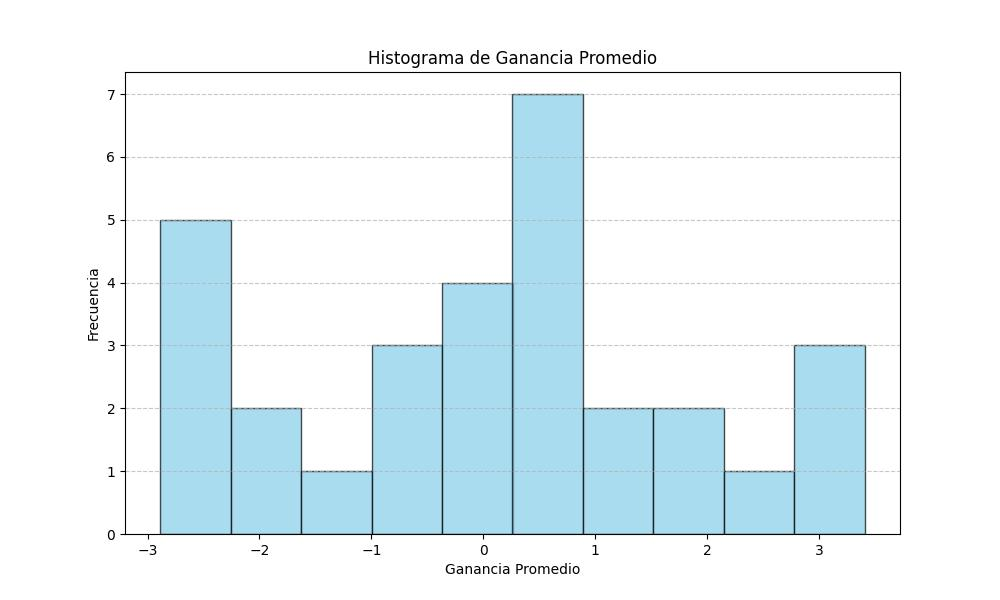
\includegraphics[width=0.8\textwidth]{./img/histograma.jpg}

La variable "Ganancia Promedio" tiene una distribución centrada en cero.
La simetría indica que las pérdidas y ganancias son comparables en frecuencia.
Los valores extremos (muy altas ganancias o muy altas pérdidas) son menos comunes

\section{Conclusiones del Modelado}
\begin{itemize}
    \item \textbf{Limitaciones del Modelo Teórico}:  
    La complejidad estocástica (demanda no Poisson, tiempos de entrega no exponenciales) dificulta soluciones analíticas exactas.
    
    \item \textbf{Ventaja de la Simulación}:  
    Permite incorporar distribuciones arbitrarias (\( G \)) y políticas complejas, proporcionando resultados empíricos robustos.
    
    \item \textbf{Validación Cruzada}:  
    Para casos simples (ej: \( G \) Poisson, \( L = 0 \)), los resultados experimentales convergen a las predicciones teóricas, confirmando la validez del modelo.
\end{itemize}


\end{document}


